% ch07 —— 第 7 章 今野宏「环簇几何与 Calabi--Yau 流形」
% 本章原书节号用阿拉伯数字（1, 2, …），而 preamble 默认 \thesection 为罗马数字。
% 原书 p.94 章末有读音标记［こんの ひろし］，按 STYLE_GUIDE §3.7 省略（记入 reports/ch07.md）。
% 章内局部改写为阿拉伯数字（与 ch04 同样处理）。
\renewcommand{\thesection}{\arabic{section}}
% ===== PDF p.092 (原书 p.84) =====
\chapter{环簇几何与 Calabi--Yau 流形}
\chapterauthor{今野宏}{[東京大学大学院数理科学研究科]}

\section{引言}

镜像对称是在 1990 年前后从超弦理论的研究中发现的。在超弦理论中，空间是 10 维的，分成 4 维时空与肉眼看不见的、极小的 6 维（即复 3 维）Calabi--Yau 流形两部分。在 4 维时空中观测到的种种量子论效应，都表现为这个 Calabi--Yau 流形几何的贡献。因此，镜像对称会预言 Calabi--Yau 流形所具有的各种几何性质。正如第 1 章中江口徹所讲解的，Candelas 等人利用镜像对称，预言了 4 维射影空间中 5 次超曲面上有理曲线的条数，给数学家带来了巨大的冲击。

Calabi--Yau 流形就是 Ricci 曲率为零的 Kähler 流形。粗略地说，Kähler 流形同时具有复结构与辛结构，而且两者满足某种相容性。第 4 章中並河良典从复流形的观点讲解了 Calabi--Yau 流形。另一方面，Calabi--Yau 流形也是辛流形。第 2 章中深谷賢治讲解的 Gromov--Witten 不变量，就是作为辛流形的不变量。所谓镜像对称，是说：给定一个 Calabi--Yau 流形时，存在另一个称为其镜像流形的 Calabi--Yau 流形，一方的复几何与另一方的辛几何相互对应。也就是说，若想研究 Calabi--Yau 流形的辛几何，只要去研究其镜像流形的复几何就行了。前面提到的 Candelas 等人的工作，也可以这样来理解：他们计算 5 次超曲面的镜像流形的周期（这是复几何的量），由此求出了 5 次超曲面的 Gromov--Witten 不变量。
% ===== PDF p.093 (原书 p.85) =====
数学中镜像对称研究的出发点，是给定 Calabi--Yau 流形之后，实际构造出它的镜像流形，并检验由镜像对称预言的事情是否真的成立。本章标题中的环簇几何，正是在这个阶段变得非常有效的手段。环簇几何是所谓环簇这种空间的几何；作为它的子流形，可以构造出 Calabi--Yau 流形。这个 Calabi--Yau 流形的性质由环簇几何来描述。而且镜像流形也能具体构造出来。本章就想说明环簇几何与镜像对称之间的这种关系。与本章相关的许多文章收在 [1] 中，感兴趣的读者请务必参阅。

\section{什么是环簇}

$n$ 维复射影空间 $\CP^n$，是把 $\C^{n+1}\setminus\{0\}$ 用 $\C^\times=\C\setminus\{0\}$ 的作用取商得到的商空间，它是一个复流形。即 $\CP^n=(\C^{n+1}\setminus\{0\})/\C^\times$。因为 $(\C^\times)^{n+1}$ 自然地作用于 $\C^{n+1}$，而且这个作用与 $\C^\times$ 的作用可交换，所以环面 $T^n_\C=(\C^\times)^{n+1}/\C^\times$ 保复结构地作用于 $\CP^n$。这时，过 $[1:1:\cdots:1]\in\CP^n$ 的环面 $T^n_\C$ 的轨道 $T^n_\C[1:1:\cdots:1]$ 在 $\CP^n$ 中稠密。因此，$\CP^n$ 是把环面 $T^n_\C$ 与其群结构相容地紧化所得的空间。这样的空间称为环簇。toric 一词似乎是意为“环面的”的生造词。

一般地，环簇 $X(\Sigma)$ 是这样构成的：从 $\C^d$ 中去掉子集 $Z(\Sigma)$，再用 $(\C^\times)^d$ 的子环面 $K_\C$ 取商\footnote{准确地说，是称为 categorical quotient 的商空间。}。即
\begin{equation}
  X(\Sigma)=(\C^d\setminus Z(\Sigma))/K_\C \tag{1}
\end{equation}
这里，集合 $Z(\Sigma)$ 与子环面 $K_\C$ 由称为扇的某种组合论数据确定。
% ===== PDF p.094 (原书 p.86) =====
下面把由扇 $\Sigma$ 给出的环簇记作 $X(\Sigma)$。这时可以验证，商环面 $T^n_\C=(\C^\times)^d/K_\C$ 作用于 $X(\Sigma)$，并且在 $X(\Sigma)$ 中有稠密的轨道。

把这些事再稍微详细地说明一下。首先考虑格 $N\cong\Z^n$，以及包含它的 $n$ 维实向量空间 $N_\R\cong\R^n$。有理多面锥 $\sigma$ 是由有限个向量 $v_1,\dots,v_s\in N$ 张成的锥
\begin{equation}
  \sigma=\Bigl\{\sum_{i=1}^{s}a_iv_i\in N_\R\Bigm|a_i\ge 0\Bigr\}\subset N_\R \tag{2}
\end{equation}
其中 $\sigma$ 还要满足 $\sigma\cap(-\sigma)=\{0\}$。$N_\R$ 内的扇 $\Sigma$ 是由有限个有理多面锥组成的集合，满足：
\begin{enumerate}[label=\arabic*.,leftmargin=2.2em,itemsep=1pt,topsep=2pt]
  \item 属于 $\Sigma$ 的有理多面锥 $\sigma$ 的面也属于 $\Sigma$；
  \item 属于 $\Sigma$ 的有理多面锥 $\sigma_1,\sigma_2$ 的公共集合 $\sigma_1\cap\sigma_2$，既是 $\sigma_1$ 的面，同时又是 $\sigma_2$ 的面。
\end{enumerate}

对应于 2 维复射影空间 $\CP^2$ 的扇 $\Sigma$ 如下。取格 $N\cong\Z^2$ 内的点
\[
  v_1=(1,0),\qquad v_2=(0,1),\qquad v_3=(-1,-1)
\]
则
\begin{equation}
  \Sigma=\{\sigma_I\mid I\subsetneq\{1,2,3\}\} \tag{3}
\end{equation}
是扇（图 1）。这里，$\sigma_I$ 为
\begin{equation}
  \sigma_I=\Bigl\{\sum_{i\in I}a_iv_i\in N_\R\Bigm|a_i\ge 0\Bigr\} \tag{4}
\end{equation}
设 $v_i=(v_{i1},v_{i2})$。这时，代数环面之间的同态映射 $\phi\colon(\C^\times)^3\to(\C^\times)^2$ 由
\begin{equation}
  \phi((z_1,z_2,z_3))=\Bigl(\prod_{i=1}^{3}z_i^{v_{i1}},\prod_{i=1}^{3}z_i^{v_{i2}}\Bigr)=(z_1z_3^{-1},z_2z_3^{-1}) \tag{5}
\end{equation}
确定。这时，把 $(\C^\times)^3$ 的子环面 $K_\C$ 定义为同态映射 $\phi$ 下单位元的原像
\begin{equation}
  K_\C=\phi^{-1}((1,1))=\{(z,z,z)\mid z\in\C^\times\} \tag{6}
\end{equation}
对 $\sigma_I\in\Sigma$，令
% ===== PDF p.095 (原书 p.87) =====
\begin{figure}[t]
  \centering
  \begin{minipage}[t]{0.47\linewidth}\centering
    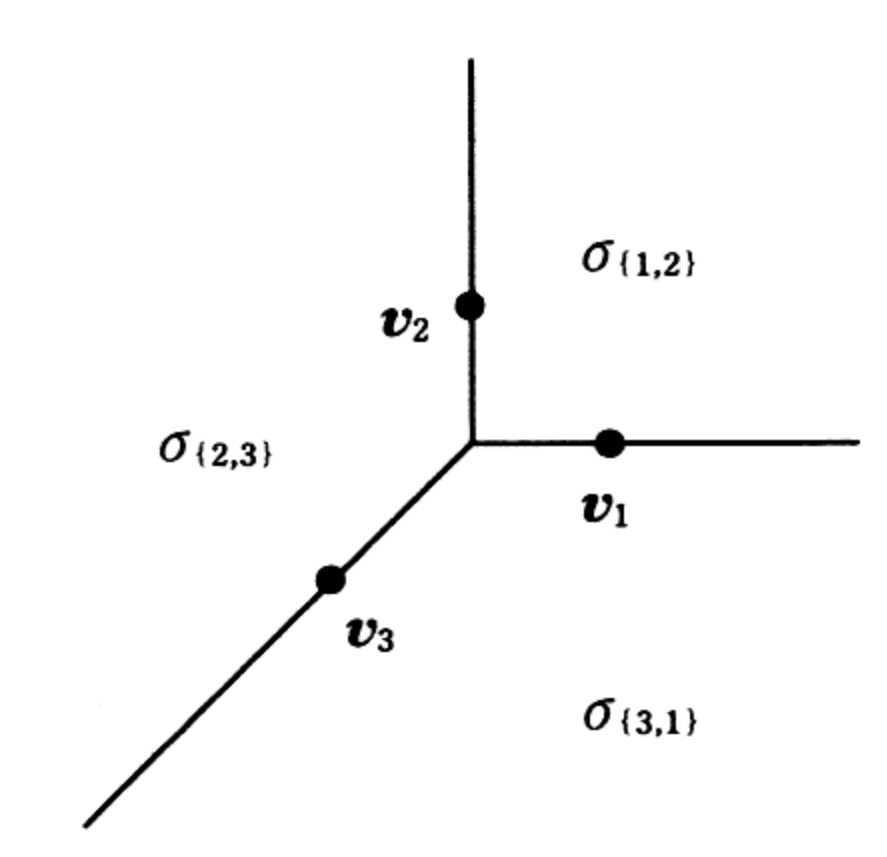
\includegraphics[height=4.0cm]{figures/ch07-fig1.png}
    \figtitle{1}{扇 $\Sigma$（原书 p.87）}
  \end{minipage}\hfill
  \begin{minipage}[t]{0.47\linewidth}\centering
    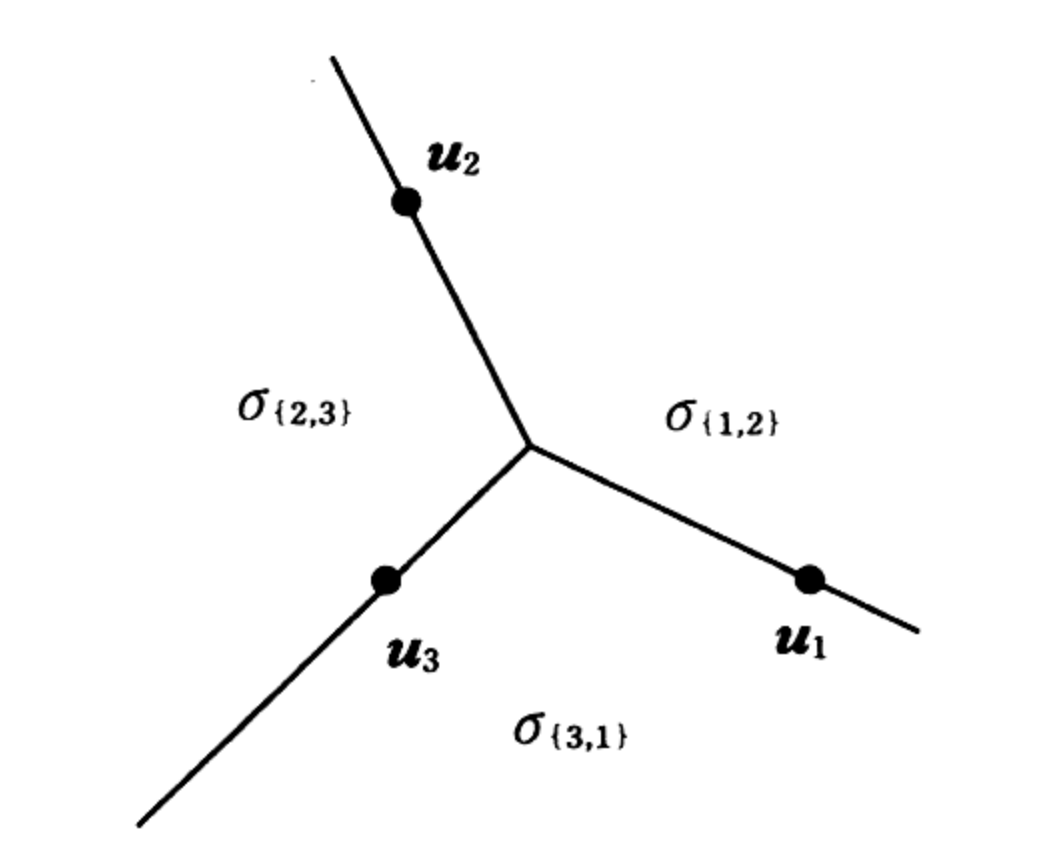
\includegraphics[height=4.0cm]{figures/ch07-fig2.png}
    \figtitle{2}{扇 $\Sigma^\circ$（原书 p.87）}
  \end{minipage}
\end{figure}

\begin{equation}
  Z(\sigma_I)=\Bigl\{(z_1,z_2,z_3)\in(\C^\times)^3\Bigm|\prod_{i\in I}z_i=0\Bigr\} \tag{7}
\end{equation}
例如 $Z(\sigma_{\{1,2\}})=\{(z_1,z_2,0)\mid z_1,z_2\in\C^\times\}$。这时定义
\begin{equation}
  Z(\Sigma)=\bigcap_{\sigma_I\in\Sigma}Z(\sigma_I) \tag{8}
\end{equation}
则 $Z(\Sigma)=\{(0,0,0)\}$。这时，
\[
  X(\Sigma)=(\C^3\setminus Z(\Sigma))/K_\C
\]
就是 $\CP^2$。并且，商环面 $T^2_\C=(\C^\times)^3/K_\C$ 作用于 $X(\Sigma)$。

又，对任意的 $\sigma_I\in\Sigma$，
\begin{equation}
  U_{\sigma_I}=(\C^3\setminus Z(\sigma_I))/K_\C \tag{9}
\end{equation}
是 $X(\Sigma)$ 的开集，具有简单的结构。例如 $U_{\sigma_{\{1,2\}}}=\{[z_1:z_2:z_3]\in X(\Sigma)\mid z_3\ne 0\}$，以 $(z_1/z_3,z_2/z_3)$ 为坐标，可知它是 $\C^2$。又，若 $\sigma_I\subset\sigma_J$，则自然有 $U_{\sigma_I}\subset U_{\sigma_J}$，并且
\begin{equation}
  X(\Sigma)=\bigcup_{\sigma_I\in\Sigma}U_{\sigma_I} \tag{10}
\end{equation}
也就是说，环簇 $X(\Sigma)$ 是把诸 $U_{\sigma_I}$ 粘合起来得到的，其粘法由扇 $\Sigma$ 的结构决定。这样一来，环簇 $X(\Sigma)$ 的各种几何性质，就能容易地描述为扇 $\Sigma$ 的组合论性质。

再举一个后面会用到的例子。取格 $N\cong\Z^2$ 内的点
\[
  u_1=(2,-1),\qquad u_2=(-1,2),\qquad u_3=(-1,-1)
\]
时（图 2），令
\begin{equation}
  \Sigma^\circ=\{\sigma_I\mid I\subsetneq\{1,2,3\}\} \tag{11}
\end{equation}
% [Tutor Note: 下文（7）式原文写作 $(z_1,z_2,z_3)\in(\C^\times)^3$，但紧接着的例子 $Z(\sigma_{\{1,2\}})=\{(z_1,z_2,0)\}$ 含有 $z_3=0$，可见原文的 $(\C^\times)^3$ 有误，当作 $\C^3$。此处照录原文，不改动。]

% ===== PDF p.096 (原书 p.88) =====
这样得到的 $\Sigma^\circ$ 也是扇。这里 $\sigma_I$ 与 (4) 同样给出。这时，同态映射 $\phi\colon(\C^\times)^3\to(\C^\times)^2$ 为
\begin{equation}
  \phi((z_1,z_2,z_3))=(z_1^2z_2^{-1}z_3^{-1},z_1^{-1}z_2^2z_3^{-1}) \tag{12}
\end{equation}
又，$K_\C=\{(z_1,z_2,z_3)\in(\C^\times)^3\mid z_1^3=z_2^3=z_1z_2z_3\}$。设 $K_\C^0$ 为 $K_\C$ 中含单位元的连通分支，请注意 $K_\C/K_\C^0\cong\Z/3\Z$。并且 $Z(\Sigma^\circ)=\{(0,0,0)\}$。因此，$X(\Sigma^\circ)=\CP^2/(\Z/3\Z)$。


\section{作为辛流形}

前节我们看了环簇作为复流形的一面。下面介绍环簇作为辛流形的一面。

流形 $M$ 上的辛结构 $\omega$，是指非退化的 2 次微分形式。对 $M$ 上的向量场 $X$，$\omega(X,\cdot)$ 是 $M$ 上的 1 次微分形式；当由 $\omega$ 确定的“向量场到 1 次微分形式”的对应是同构对应时，称 $\omega$ 为非退化。李群 $G$ 保辛结构 $\omega$ 地作用于 $M$ 时，所谓辛商，指 $M$ 的由 $G$ 给出的一个特殊商空间，其定义如下。$G$ 作用于 $M$ 时，李代数\footnote{给 $G$ 的单位元处的切空间赋予称为 Lie 括号积的代数结构，就得到李代数。} $\mathfrak{g}$ 的元素 $X$ 确定 $M$ 上的向量场 $X$。这时，$G$ 等变的映射 $\mu_G\colon M\to\mathfrak{g}^*$ 若对任意 $X\in\mathfrak{g}$ 满足 $\omega(X,\cdot)=-\rd\langle\mu_G(\cdot),X\rangle$，就称为矩映射。这里 $\langle\cdot,\cdot\rangle\colon\mathfrak{g}^*\times\mathfrak{g}\to\R$ 是自然的配对，$\langle\mu_G(\cdot),X\rangle$ 是 $M$ 上的函数，$\rd$ 是外微分算子。这时 $\mu_G^{-1}(0)/G$ 具有自然的辛结构。这个商空间称为辛商。

前节说明了环簇
\[
  X(\Sigma)=(\C^d\setminus Z(\Sigma))/K_\C
\]
其中 $K_\C$ 是代数环面 $(\C^\times)^d$ 的子环面。令 $S^1=\{z\in\C\mid |z|=1\}\subset\C^\times$ 时，实环面 $(S^1)^d\subset(\C^\times)^d$ 保 $\C^d$ 的标准辛结构 $\omega$ 地作用。这时，在很多情况下 $X(\Sigma)$ 是 $\C^d$ 的实子环面 $K=(S^1)^d\cap K_\C$ 的辛商。也就是说，若适当取矩映射 $\mu_K\colon\C^d\to\mathfrak{k}^*$，则
% [Tutor Note: 其一，$\CP^2/(\Z/3\Z)$ 有不动点，这里取的是轨形（orbifold）意义下的商；相应地 $X(\Sigma^\circ)$ 作为簇带有商奇点，与第 4 节的反射多面体构造正好接上。其二，上文把辛结构写成“非退化的 2 次微分形式”，非退化到下一句才解释；原书此处未提闭性 $\mathrm{d}\omega=0$，通常的辛形式定义还要求闭，译文照录。]

% ===== PDF p.097 (原书 p.89) =====
\begin{equation}
  X(\Sigma)=(\C^d\setminus Z(\Sigma))/K_\C=\mu_K^{-1}(0)/K \tag{13}
\end{equation}
并且，实商环面
\[
  T^n=(S^1)^d/K\subset T^n_\C=(\C^\times)^d/K_\C
\]
保 $X(\Sigma)$ 上的辛结构地作用。这个作用的矩映射 $\mu_{T^n}\colon X(\Sigma)\to(\mathfrak{t}^n)^*$ 的像 $\Delta=\Image\mu_{T^n}\subset(\mathfrak{t}^n)^*$ 是凸多面体。这里 $\mathfrak{t}^n$ 是商环面 $T^n=(S^1)^d/K$ 的李代数，它自然与 $N_\R$ 等同。因此，凸多面体 $\Delta$ 是 $(\mathfrak{t}^n)^*=(N_\R)^*$ 的子集。由这个凸多面体 $\Delta\subset(N_\R)^*$，可以重构扇 $\Sigma\subset N_\R$，从而重构 $X(\Sigma)$。而且 $X(\Sigma)$ 上的辛结构也能重构。以后，把由凸多面体 $\Delta$ 确定的环簇记作 $X(\Delta)$。

这样一来，环簇是同时具有复几何侧面与辛几何侧面的空间。所以，环簇在镜像对称中扮演重要角色，也许是自然而然的。

\section{Fano 流形的构造}

复流形 $M$ 若其第一 Chern 类 $c_1(M)\in H^2(M;\R)$ 为正，就称为 Fano 流形；换言之，第一 Chern 类为正，是指它可由与复结构相容的辛形式代表。这时，反典范除子\footnote{反典范丛 $K_M^{-1}$，即满足 $c_1(K_M^{-1})=c_1(M)$ 的 $M$ 上的全纯线丛，其全纯截面的零点所表示的 $M$ 的超曲面。}只要没有奇点，就成为 Calabi--Yau 流形。

我们一直在考虑格 $N\cong\Z^n$，以及包含它的 $n$ 维实向量空间 $N_\R\cong\R^n$。这时，对偶格 $N^*\cong\Z^n$，以及包含它的 $n$ 维实向量空间 $(N_\R)^*\cong\R^n$ 就确定了。凸多面体 $\Delta\subset(N_\R)^*$ 的极对偶 $\Delta^\circ\subset N_\R$ 是由
\begin{equation}
  \Delta^\circ=\bigl\{v\in N_\R\bigm|\text{对任意 }u\in\Delta,\ \langle u,v\rangle\ge -1\bigr\} \tag{14}
\end{equation}
% ===== PDF p.098 (原书 p.90) =====
所确定的凸多面体。顶点落在对偶格 $N^*$ 中的凸多面体 $\Delta\subset(N_\R)^*$ 称为反射多面体：$(N_\R)^*$ 的原点位于 $\Delta$ 的内部，并且极对偶 $\Delta^\circ\subset N_\R$ 的顶点都是 $N$ 的点。由反射多面体 $\Delta$ 确定的环簇 $X(\Delta)$，是具有某种奇点的 Fano 流形。而且，$\Delta$ 所确定的 $X(\Delta)$ 的辛结构是 $c_1(X(\Delta))\in H^2(X(\Delta);\R)$ 的代表元。

现在，2 维复射影空间 $\CP^2$ 是 Fano 流形；确定这个空间的凸多面体 $\Delta\subset(N_\R)^*$ 的顶点是
\[
  u_1=(2,-1),\qquad u_2=(-1,2),\qquad u_3=(-1,-1)\in N^*\cong\Z^2
\]
（图 3）。$\Delta$ 的极对偶 $\Delta^\circ\subset N_\R$ 的顶点为 $v_1=(1,0)$，$v_2=(0,1)$，$v_3=(-1,-1)$（图 4），可知 $\Delta$ 是反射多面体。第 2 节中我们从这些向量出发，构成了确定 $\CP^2$ 的扇 $\Sigma$；$\Delta^\circ$ 的顶点与属于 $\Sigma$ 的 1 维有理多面锥（这里是以原点为起点的半直线）相对应。而且，$\Delta^\circ$ 的边与属于 $\Sigma$ 的 2 维有理多面锥相对应。这样，确定 $X(\Delta)=\CP^2$ 的扇 $\Sigma$，就实现为极对偶 $\Delta^\circ$ 上的锥。以上归纳起来就是：$\CP^2=X(\Sigma)=X(\Delta)$，而 $\Sigma$ 是 $\Delta^\circ$ 上的锥。

现在把这个例子中的 $N$ 与 $N^*$ 的立场对调一下。考虑 $\Delta^\circ\subset N_\R$ 的极对偶 $(\Delta^\circ)^\circ\subset(N_\R)^*$，则 $(\Delta^\circ)^\circ=\Delta$。因此 $\Delta^\circ$ 也是反射多面体。而且，对应于环簇 Fano 流形 $X(\Delta^\circ)$ 的扇，是 $(\Delta^\circ)^\circ=\Delta$ 上的锥，所以这恰好就是第 2 节最后所述的例子 $\Sigma^\circ$。即 $X(\Delta^\circ)=X(\Sigma^\circ)=\CP^2/(\Z/3\Z)$。

如上所述，给定反射多面体 $\Delta$，就得到环簇 Fano 流形 $X(\Delta)$；与此同时，从极对偶 $\Delta^\circ$ 还能得到另一个环簇 Fano 流形 $X(\Delta^\circ)$。

\begin{figure}[t]
  \centering
  \begin{minipage}[t]{0.47\linewidth}\centering
    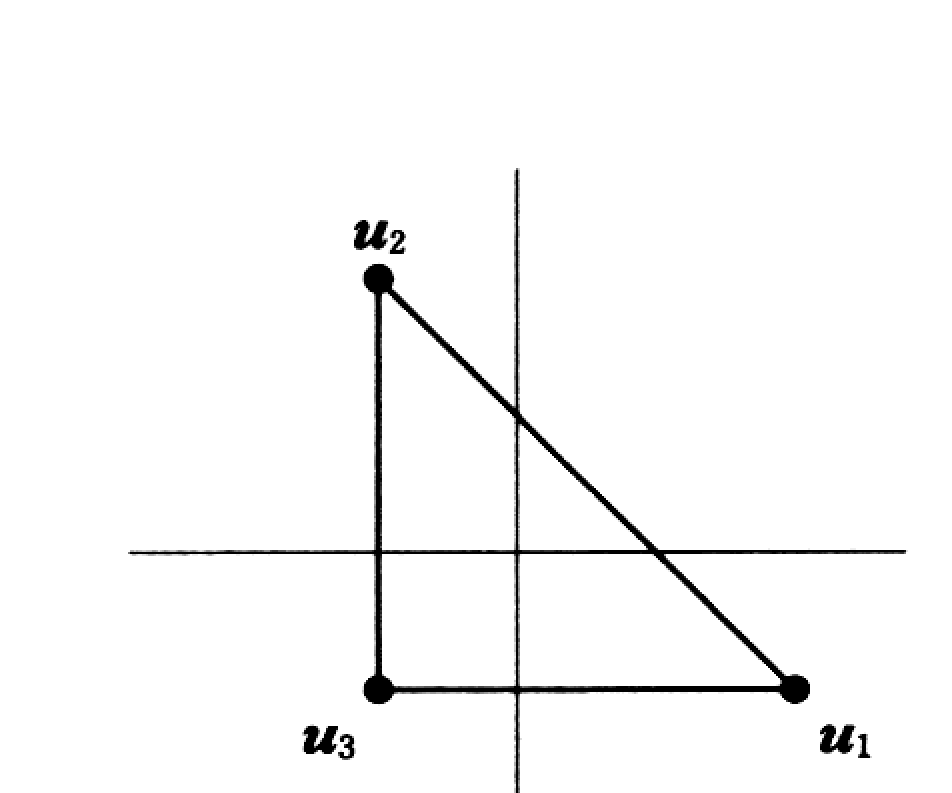
\includegraphics[height=4.0cm]{figures/ch07-fig3.png}
    \figtitle{3}{反射多面体 $\Delta$（原书 p.90）}
  \end{minipage}\hfill
  \begin{minipage}[t]{0.47\linewidth}\centering
    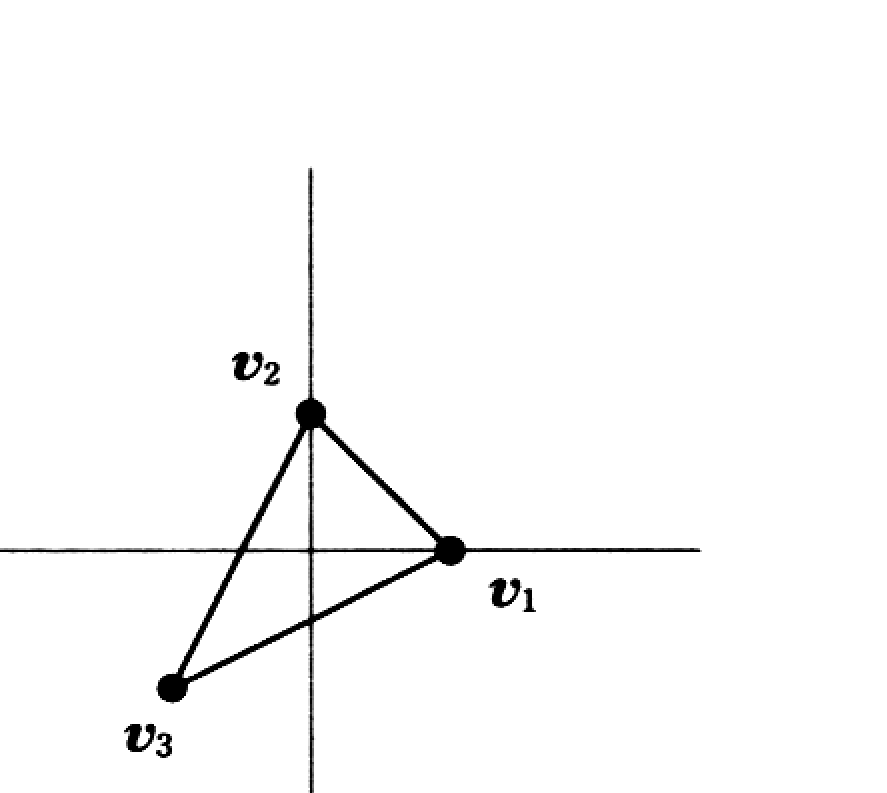
\includegraphics[height=4.0cm]{figures/ch07-fig4.png}
    \figtitle{4}{极对偶 $\Delta^\circ$（原书 p.90）}
  \end{minipage}
\end{figure}
% ===== PDF p.099 (原书 p.91) =====
人们期待从 $X(\Delta)$ 的反典范除子得到 Calabi--Yau 流形；但一般来说，$X(\Delta)$ 有奇点，其超曲面也有奇点。不过，这些奇点可以按某种自然的方式至少部分地消解，从而得到 Calabi--Yau 流形 $M$。特别是在 3 维情形，可以得到没有奇点的 Calabi--Yau 流形。另一方面，消解 $X(\Delta^\circ)$ 的反典范除子的奇点，得到 Calabi--Yau 流形 $M^\circ$。实际上，人们期待这个 $M$ 与 $M^\circ$ 互为镜像流形。事实上，当 $M$ 是 3 维时，
\begin{equation}
  h^{2,1}(M)=h^{1,1}(M^\circ),\qquad h^{1,1}(M)=h^{2,1}(M^\circ) \tag{15}
\end{equation}
成立。这个事实称为拓扑镜像对称，是镜像对称所预言的最基本的事实。


Green 与 Plesser 在物理考察的基础上指出：对 4 维射影空间的 5 次超曲面等，通过用有限群取商，可以构造出镜像流形。Batyrev 把这种构造法放到环簇几何的框架中重新理解，发现了上述构造镜像流形的方法，并证明了 (15)。事实上，以
\[
  \begin{gathered}
    v_1=(4,-1,-1,-1),\qquad v_2=(-1,4,-1,-1),\\
    v_3=(-1,-1,4,-1),\qquad v_4=(-1,-1,-1,4),\\
    v_5=(-1,-1,-1,-1)
  \end{gathered}
\]
为顶点的凸多面体 $\Delta\subset(N_\R)^*\cong\R^4$ 是反射多面体；应用这个构造法，得到
\[
  X(\Delta)=\CP^4,\qquad X(\Delta^\circ)=\CP^4/(\Z/5\Z)^3
\]
$\CP^4$ 的反典范除子是 5 次超曲面。作为 $\CP^4/(\Z/5\Z)^3$ 的反典范除子的奇点消解，得到 5 次超曲面的镜像流形。

Batyrev 的构造法使我们能够系统地构造镜像流形。这一构造法被推广到环簇的完全交等情形，得到了许多互为镜像流形的 Calabi--Yau 流形对。

\section{镜像对称}

如上所述，镜像流形——更准确地说，是期待成为镜像流形的东西——已经构造出来；接下来应该做的，是对它们验证镜像对称所预言的事实。设 $M$ 为 3 维 Calabi--Yau 流形，我们来想一想 (15) 的意义。
% [Tutor Note: （15）的两式把 Hodge 数 $h^{1,1}$ 与 $h^{2,1}$ 互换：辛几何一侧的 Kähler 形变参数与复几何一侧的复结构形变参数维数相等。这正是「镜像」一词的拓扑含义，也是检查一个候选镜像对是否合格的第一道门槛。]

% ===== PDF p.100 (原书 p.92) =====
$h^{2,1}(M^\circ)$ 是 $M$ 的镜像流形 $M^\circ$ 的复结构形变空间 $\cM_{\mathrm{cpx}}(M^\circ)$ 的维数。另一方面，$h^{1,1}(M)$ 是 $M$ 的（复化后的）Kähler 度量的形变空间 $\cM_{\mathrm{kah}}(M)$，也就是 $M$ 的辛结构的形变空间的维数。(15) 主张这两个空间的维数相等。

$\cM_{\mathrm{kah}}(M)$ 中存在一个称为 large radius limit（大半径极限）的无穷远点。另一方面，$\cM_{\mathrm{cpx}}(M^\circ)$ 中存在称为 large complex structure limit（大复结构极限）的无穷远点。镜像对称的主张是：这些无穷远点的邻域之间存在自然的同构映射。这个称为镜像变换的同构映射，按下面的方式把 $M^\circ$ 的辛几何与 $M^\circ$ 的复几何对应起来。
% [Tutor Note: 此处第一个 $M^\circ$ 疑为 $M$，译文照录。]
首先，这些无穷远点的邻域各自具有某种自然的坐标系，而且它们在镜像变换下相互对应。进一步，$M$ 所确定的 A 模型的 Yukawa 耦合，与 $M^\circ$ 所确定的 B 模型的相应 Yukawa 耦合，在这个镜像变换下相等。以上就是经典镜像对称的主张。$M$ 所确定的 A 模型的 Yukawa 耦合，是由 $M$ 的有理曲线条数——更准确地说，是由 $M$ 的亏格 0 的 Gromov--Witten 不变量——确定的量，由 $M$ 的辛几何确定。另一方面，$M^\circ$ 所确定的 B 模型的 Yukawa 耦合，是由 $M^\circ$ 的周期积分确定的复几何量。第 1 章讲解过的 Candelas 等人的工作，是在 $M$ 为 5 次超曲面的情形具体描述这个镜像变换，并进一步具体计算 $M^\circ$ 所确定的 B 模型的 Yukawa 耦合；由此预言 $M$ 所确定的 A 模型的 Yukawa 耦合的值。

当 Calabi--Yau 流形 $M$ 作为环簇 Fano 流形 $X(\Delta)$ 的反典范除子的奇点消解得到时，其镜像流形 $M^\circ$ 是通过消解 $X(\Delta^\circ)$ 的反典范除子的奇点得到的。这时，$\cM_{\mathrm{kah}}(M)$ 中的 large radius limit，可以容易地由 $X(\Delta)$ 的几何来描述。另一方面，$\cM_{\mathrm{cpx}}(M^\circ)$ 可以基于 $X(\Delta^\circ)$ 的反典范丛的全纯截面空间来描述。$M^\circ$ 的周期积分是 $\cM_{\mathrm{cpx}}(M^\circ)$ 上的全纯函数，已知它满足称为 GKZ（Gelfand--Kapranov--Zelevinsky）方程组的微分方程组。

% ===== PDF p.101 (原书 p.93) =====
large complex structure limit 这个无穷远点，是这个周期积分的单值性（monodromy）的最大退化点；通过研究这个微分方程组就能找到。进一步，利用这个微分方程组的解，可以构成该无穷远点邻域中的自然坐标系，并求出镜像变换与 B 模型的 Yukawa 耦合。这样，B 模型就能用成熟的传统复几何手法来研究。另一方面，对 A 模型来说，曾有建立 Gromov--Witten 不变量理论等重要问题；但终于在 1996 年前后，先是 Givental、随后是 Lian--Liu--Yau，利用环面作用成功求出了 A 模型的 Yukawa 耦合。这样，当 Calabi--Yau 流形 $M$ 作为环簇 Fano 流形 $X(\Delta)$ 的反典范除子的奇点消解得到时，通过分别计算 A 模型、B 模型的 Yukawa 耦合，经典镜像对称的主张得到了证明。

\section{SYZ 猜想}

第 4 节说明了如何构造作为环簇反典范除子的奇点消解而得到的 Calabi--Yau 流形 $M$ 的镜像流形 $M^\circ$。这个方法很具体，实际计算时非常方便；但由于是用环簇几何的语言描述的，$M$ 与 $M^\circ$ 的内在关系看不太清楚。Strominger--Yau--Zaslow 提出了从 $M$ 构造 $M^\circ$ 的如下方法：$M$ 在 large complex structure limit 附近具有由半维环面构成的纤维化结构；而 $M^\circ$ 实现为其对偶环面的纤维化的全空间。这个方法称为 SYZ 猜想（构造），是表达 $M$ 与 $M^\circ$ 内在关系的有力工具。进一步，还要求纤维环面是特殊 Lagrangian 子流形；或者只要求纤维在趋近 large complex structure limit 时渐近地接近特殊 Lagrangian 子流形；这在微分几何上也是很有意思的猜想。不过，这个环面纤维化的奇异纤维的结构还没有得到很好的理解，所以这一构造法在数学上还没有充分形式化。本来这个猜想基于“镜像对称就是 T 对偶”这一物理考察，
% [Tutor Note: “T 对偶”指半径 $R$ 的圆周与半径 $1/R$ 的圆周给出同一个物理的理论，是弦论中最早被认识的等价性；SYZ 猜想把镜像对称解释为沿纤维环面的 T 对偶。第 6 章会从共形场论的角度再讲这件事。]

% ===== PDF p.102 (原书 p.94) =====
这一考察在第 6 章中由細野忍详细讲解。

当 Calabi--Yau 流形 $M$ 由环簇 $X(\Delta)$ 的超曲面构成时，这样的环面纤维化已由 Ruan、Zharkov 等人构造出来。这个环面纤维化接近于把 $X(\Delta)$ 的矩映射 $\mu_{T^n}\colon X(\Delta)\to(\mathfrak{t}^n)^*$ 限制到 $M$ 上。$X(\Delta)$ 的超曲面在 $\mu_{T^n}$ 下的像呈现某种阿米巴（amoeba）的形状，数学中也确实使用这个名称。阿米巴与镜像对称、热带几何、实代数几何等相联系，相关研究现在十分活跃。

\section{结语}

这样，超弦理论中发现的镜像对称，随着大量例子被构造出来，在数学上也逐渐站住了脚。然而上面经典镜像对称的证明，只是分别计算两个量，结果发现这两个量相等，并没有弄清它们相等的根本理由。而且，经典镜像对称只陈述了 $M$ 的辛几何与 $M^\circ$ 的复几何对应关系的一个侧面。Kontsevich 从范畴论立场重新理解镜像对称，给出了更根本的形式化。这称为同调镜像对称，相关研究现在十分活跃。关于这一点，第 8 章、第 10 章有叙述。

\begin{reflist}
  \item[{[1]}] 特集「トーリック多様体」，『数学セミナー』2004 年 3 月号．
  \item[{[2]}] D. Cox and S. Katz, \textit{Mirror Symmetry and Algebraic Geometry}, 1999, AMS.
\end{reflist}

% 本章节号至此结束，恢复 preamble 的罗马数字默认，避免影响 ch08 及以后。
\renewcommand{\thesection}{\Roman{section}}